\chapter{Tecnologie}
In questo capitolo verranno descritte le attività preliminari per la realizzazione di questo progetto, le tecnologie utilizzate
unitamente alle motivazioni legate all'uso di questi sistemi rispetto ad altri.

\section{Gestire dati in modo gerarchico}
The tables of a relational database are not hierarchical (like XML), but are simply a flat list. Hierarchical data has a parent-child 
relationship that is not naturally represented in a relational database table. Hierarchical data is a collection of data where each item 
single parent and zero or more children (with the exception of the root item, which has no parent). Hierarchical data can be found in 
a variety of database applications, including forum and mailing list threads, business organization charts, content management 
categories, and product categories.
\begin{figure}[!htbp]
    \centering
	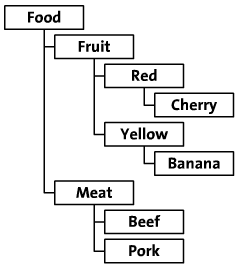
\includegraphics[scale=0.7]{images/Hierarchical_Data_ex.PNG}
	\caption{Esempio di una gestione di dati in modo gerarchico}
\end{figure}

\newpage

There are different models for dealing with hierarchical data:

\subsection{The adjacency list model}
The first, and most elegant, approach we’ll try is called the ‘adjacency list model’ or the ‘recursion method’. It’s an elegant approach 
because you’ll need just one, simple function to iterate through your tree.

In the adjacency list model, each item in the table contains a pointer to its parent. The topmost element has a NULL value for its parent.
The adjacency list model has the advantage of being quite simple, it is easy to see the children of a node. 

CONS:
While the adjacency list model can be dealt with fairly easily in client-side code, working with the model can be more problematic in 
pure SQL.

In most programming languages, it’s slow and inefficient. This is mainly caused by the recursion. We need one database query for each 
node in the tree.
As each query takes some time, this makes the function very slow when dealing with large trees.

\subsection{The nested set model}
In the Nested Set Model, we can look at our hierarchy in a new way, not as nodes and lines, but as nested containers. 

\begin{figure}[!htbp]
    \centering
	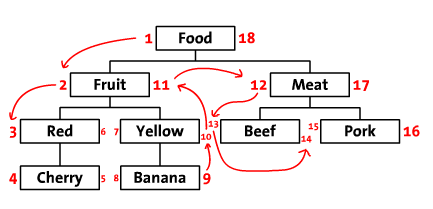
\includegraphics[scale=1]{images/Nested_Tree_Model_ex.PNG}
	\caption{Esempio di una gestione di dati in modo gerarchico secondo il modello innestato}
\end{figure}

\newpage

We represent this form of hierarchy in a table through the use of left and right values to represent the nesting of our nodes, 
and indicate the relationship between each node.
So how do we determine left and right values? 
We start numbering at the leftmost side of the outer node and continue to the right. When working with a tree, we work from left to 
right, one layer at a time, descending to each node’s children before assigning a right-hand number and moving on to the right. 
This approach is called the modified preorder tree traversal algorithm.

\begin{figure}[!htbp]
    \centering
	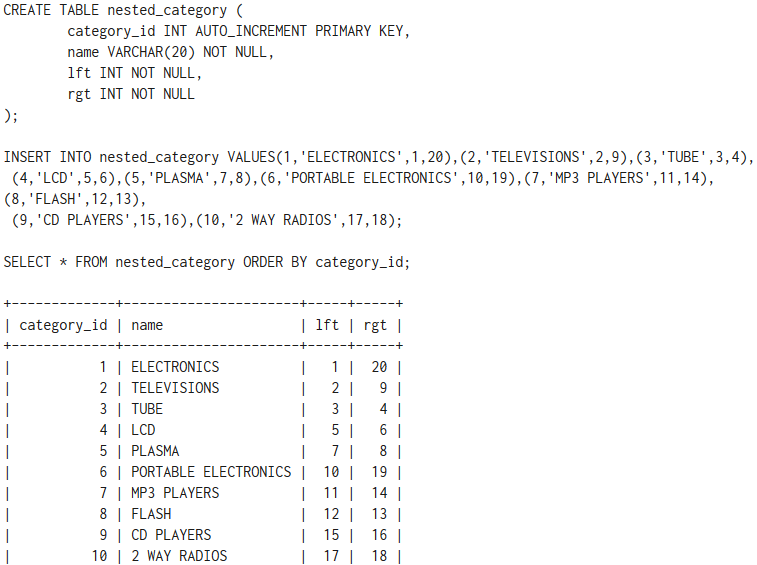
\includegraphics[scale=1]{images/Nested_Tree_Model_table.PNG}
	\caption{Esempio di una tabella per gestire dati in modo gerarchico secondo il modello innestato}
\end{figure}

OSS: Note that the words ‘left’ and ‘right’ have a special meaning in SQL. Therefore, we’ll have to use ‘lft’ and ‘rgt’ to identify 
the columns. Also note that we don’t really need the ‘parent’ column anymore. We now have the lft and rgt values to store the tree 
structure.

CONS: At first, the modified preorder tree traversal algorithm seems difficult to understand. It certainly is less simple than the 
adjacency list method. However, once you’re used to the left and right properties, it becomes clear that you can do almost everything 
with this technique that you could do with the adjacency list method, and that the modified preorder tree traversal algorithm is much 
faster. Updating the tree takes more queries, which is slower, but retrieving the nodes is achieved with only one query.


\section{Sistemi di raccomandazione}